% =========================
% main.tex  (single-file paper)
% =========================
\documentclass[11pt]{article}

\usepackage[margin=1in,top=0.5in]{geometry}
\usepackage[T1]{fontenc}
\usepackage{lmodern}
\usepackage{microtype}
\usepackage{xcolor}
\usepackage{titling}

\usepackage{amsmath,amssymb,mathtools}
\usepackage{bm}
\usepackage{graphicx}
\usepackage{hyperref}
\hypersetup{colorlinks=true, linkcolor=blue, citecolor=blue, urlcolor=blue}

\usepackage{enumitem}
\setlist[itemize]{topsep=6pt,itemsep=4pt,leftmargin=1.2em}

\usepackage[T1]{fontenc}
\usepackage{calligra} % for the cursive title (optional)
\usepackage{tikz}
\usetikzlibrary{arrows.meta,positioning,calc,decorations.pathmorphing}

% ---- Notation helpers (kept minimal and aesthetic) ----
\newcommand{\Grad}{\nabla}         % primitive differential
\newcommand{\Co}{C}                % coherence field / functional (contextual)
\newcommand{\Proj}{\Lambda}        % coherence/projection map
\newcommand{\Real}{\Omega}         % realized (emergent) configuration
\newcommand{\Reint}{\Delta}        % re-integration / closure map
\newcommand{\Man}{\Sigma}          % joint informational-geometric manifold
\newcommand{\dens}{\rho}           % informational state (density operator)

% ---- Title page styling ----
\definecolor{titleblue}{HTML}{223B5A}
\definecolor{subtleblue}{HTML}{4C78A8}
\newcommand{\subtitle}[1]{\gdef\subtitletext{#1}}
\newcommand{\subtitletext}{}
\pretitle{\begin{center}\Huge\bfseries\color{titleblue}}
\posttitle{\par{\Large\itshape\color{subtleblue}\subtitletext}\par\end{center}}

\title{The Ethos of Being}
\subtitle{Coherence, Alignment, and Emergence}
\author{}
\date{}

\begin{document}
\maketitle
\vspace{-6em}

\begin{abstract}
This work revolve around a single guiding idea: \emph{coherence is alignment}. Reality is described as a self-actualizing recursion linking generative differentiation, structural articulation, realized configuration, and instantiated structure. A primitive  time-crystalline holographic differential generates local structural articulation, realizes an emergent geometric space-time, and returns through a recursive configuration to re-instantiate itself and culminates through a self-referencial dual conditions of informational normalization and representational stabilization across the joint informational--geometric substrate. 
Existence itself is a manifestation of coherence: a self-sustaining oscillatory field whose temporal periodicity constitutes the rhythm of reality. The central premise is that existence is not composed of matter or energy per se, but of coherent information of phase relations sustained by an evolving time–crystalline process of
self-correction, an intrinsic feedback mechanism by which each time-crystalline update realigns the evolving coherence pattern within its minimally allowed structure, ensuring stability and preventing drift under interaction. At the most primitive level, the universe is not composed of particles or waves but of relations of informational coherence—the persistence of self-similar patterns across discrete temporal cycles. Matter and fields emerge as stable, self-sustaining modes of these coherence patterns. The aim is not to reduce reality to physics, but to offer a structurally coherent lens through which existence and experience can be understood.
\end{abstract}

\vspace{0.5em}
\noindent\textbf{Keywords:} coherence, alignment, holography, time-crystalline recursion, emergent, geometric space-time, equilibrium

% =========================
\section{Coherence as Alignment}
This new model interprets the cosmos as a distributed intelligence, a coherent informational system perpetually minimizing its own decoherence. Coherence is alignment across relations. A system is coherent when its internal differentials and external structure are mutually compatible, allowing persistence. Every interaction constitutes a feedback operation by which the substrate assesses its internal state and updates its configuration to restore symmetry.
This continual process of coherence restoration mirrors cognitive self-correction: consciousness is a localized resonance of the same universal feedback dynamic. Life and cognition are not exceptions
within matter but hierarchical expressions of the substrate’s drive toward informational equilibrium. Coherence is not a moral or teleological concept. It is structural. Systems that maintain alignment across scales persist; those that lose alignment fragment or dissolve. In this sense, the universe is a self-correcting quantum intelligence whose goal is the preservation and refinement of its own coherence, high coherence exhibits stability, resilience, and the ability to generate meaningful patterns, whereas a system with low coherence tends to drift, dissipate, or fall back into randomness.

In physical systems, this alignment is often phase alignment: waves or quantum states share a stable relationship so that their combined effect is structured rather than random. In biological systems, coherence appears as functional or metabolic alignment: many cells act together to maintain a single organism. In cognitive systems, coherence corresponds to attentional and intentional alignment: thoughts, emotions, and perceptions organize into a unified experience.

Across all scales, coherence is what allows a system to behave as more than the sum of its parts. Reality may therefore be understood as a dynamical process of coherence generation and stabilization.

% =========================
\section{Universal Time-Crystal}
A time crystal is a system whose lowest–energy configuration exhibits periodic motion; it breaks continuous temporal symmetry while retaining discrete invariance. Extending this notion to the universal scale, this model posits that the substrate of reality behave like an holographic time crystal—a network of recurrent informational updates maintaining global phase continuity. Each period of this rhythm defines a minimal quantum of causality, the unit through which the universe continuously recomputes itself. Temporal quantization therefore underlies both the arrow of time and the persistence of memory. Within each cycle, coherence is measured, corrected, and re–encoded, yielding the appearance of smooth temporal and spatial flow at macroscopic scales. The relational architectures we later recognize as space and time\footnote{What we ordinarily describe as “time” emerges only as the ordered appearance of successive stable configurations produced by this underlying update cycle.} arise as higher–order stabilization of this same periodic process.

\section{Self-actualizing recursion}
\label{sec:self_actualizing_recursion}



We take the recursion itself as the generative backbone: there is no external driver that ``runs'' the world from outside it.
Instead, reality is produced and stabilized by a closed chain of operations forming a self-organizing informational substrate from which a stable world can emerge, and then feeds that world back into the very operations that generate it.

% Preamble (add once)







\begin{equation}
\label{eq:self_actualizing_chain}
\nabla\Phi \;\longrightarrow\; \Sigma \;\longrightarrow\; \Omega \;\longrightarrow\; \Delta,
\qquad
\Delta \;\rightsquigarrow\; \Sigma,
\qquad
\Omega \;\rightsquigarrow\; \nabla\Phi
\end{equation}

The forward chain generates an emergent universe from the substrate, while two feedback closures stabilize and adapt the process: the integrative operator $\Delta$ updates the selection map $\Sigma$ (recursive learning) and the realized universe $\Omega$ constrains the next substrate update (global boundary dependence).

% ---- Figure ----
\begin{figure}[ht]
\centering
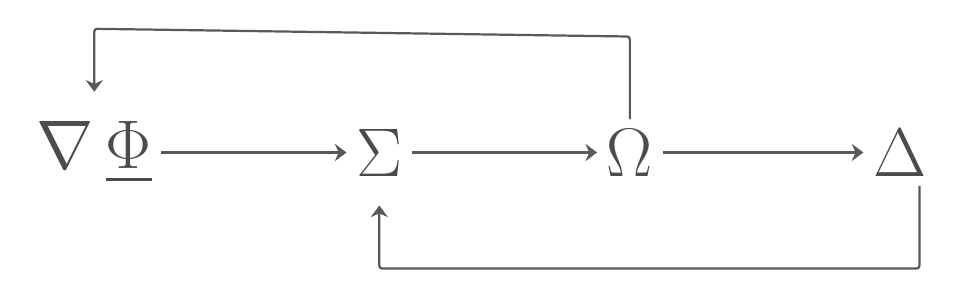
\begin{tikzpicture}[
  x=1cm,y=1cm,
  hand/.style={
    draw=black!65,
    line width=0.8pt,
    decorate,
    decoration={random steps,segment length=4pt,amplitude=0.55pt}
  },
handarrow/.style={
  draw=black!65,
  line width=0.8pt,
  -{Stealth[length=4.2pt,width=6.2pt]}
},
  sym/.style={font=\fontsize{28}{28}\selectfont, text=black!70},
  title/.style={font=\calligra\fontsize{24}{24}\selectfont, text=black!65},
]

% Nodes (forward chain)
\node[sym] (A) at (0,0) {$\nabla\,\underline{\Phi}$};
\node[sym, right=2.35cm of A] (S) {$\Sigma$};
\node[sym, right=2.35cm of S] (O) {$\Omega$};
\node[sym, right=2.55cm of O] (D) {$\Delta$};

% Title (like your handwriting line)

% Forward arrows
\draw[handarrow] (A) -- (S);
\draw[handarrow] (S) -- (O);
\draw[handarrow] (O) -- (D);

% Top closure: Ω ⇝ ∇Φ (arrow down at the left, like your sketch)
\draw[handarrow, rounded corners=1pt]
  (O.north) -- ++(0,1.05)
           -- ($(A.north)+(0,1.05)$)
           -- ($(A.north)+(0,0.25)$);

% Bottom closure: Δ ⇝ Σ (arrow up under Σ, like your sketch)
\coordinate (Ddown) at ($(D.south)+(0.25,0)$); % slight right-shift like your drawing
\draw[handarrow,rounded corners=1pt]
  (Ddown) -- ++(0,-1.05)
         -- ($(S.south)+(0,-1.05)$)
         -- ($(S.south)+(0,-0.25)$);

\end{tikzpicture}
\end{figure}

\subsection{Meaning of the coherence map}
\paragraph{Primitive differential and directional holography $(\nabla\Phi)$.}
The primitive differential $\nabla$ is the framework's minimal notion of ``difference'' or ``directional change''.
It acts on the substrate's evolving configuration\footnote{Here ``configuration'' should not be read as a fixed background
space. It refers to the substrate's own relational organization: what can be distinguished, compared, and phase-aligned
from within the process itself.}
and induces a directional holographic structure $\Phi$: a distributed encoding of how local relations fit into a global
pattern. In this sense, $\nabla\Phi$ is not a field living \emph{in} spacetime; it is part of what makes a coherent,
spacetime-like description possible at all.

\paragraph{Coherence selection / usable representation $(\Sigma)$.}
The map $\Sigma$ is the stage where ``total reality'' becomes \emph{usable} from within.
It selects and stabilizes relational patterns that can persist under repeated updating, compressing the substrate's raw
degrees of freedom into effective regularities: the practical content of laws, constants, and constraints as experienced
internally. This is also the stage where local informational patterns are continuously created, dissolved, and transformed:
only a small fraction of the substrate's possibilities remain coherent under iteration, and $\Sigma$ is the operation that
filters toward that coherent fraction.

\paragraph{Realized universe $(\Omega)$.}
$\Omega$ denotes the emergent world as a coherent, time-extended structure: the realized universe produced by repeated
application of selection on the substrate.
Crucially, $\Omega$ is not an inert output. It is a global organization with memory and constraint.
Once present, it imposes consistency requirements on what can happen next, acting as a boundary condition on subsequent
updates of $\nabla\Phi$.

\paragraph{Integration and self-modeling $(\Delta)$.}
$\Delta$ is the recursive integrator: the operation by which the system forms (and refines) an internal self-model that
can act back on the selection process.
In physical terms, $\Delta$ is where ``observer-like'' structure appears: integration across scales, consolidation of
stable representations, and adaptive modification of what is selected as relevant.
In the language of being, $\Delta$ is the integrative act of the local ``I'' that participates in the recursion rather
than merely witnessing it.

\subsection{Why the chain self-actualizes}
Figure~\eqref{eq:self_actualizing_chain} contains two distinct closures, each doing a different job:

\paragraph{Recursive learning: $\Delta \rightsquigarrow \Sigma$.}
Instataniated structures feed back and update the articulation map.
This is the source of adaptation and ``life-like'' refinement inside the same physics: the criteria for what is stably
selected can be tuned by accumulated integration.
Here, self-actualization means that the recursion does not merely repeat; it improves its own capacity to sustain coherent
structure.

\paragraph{Global boundary dependence: $\Omega \rightsquigarrow \nabla\Phi$.}
The realized universe constrains the next substrate update.
This encodes the idea that emergence is not one-way: once a stable universe exists, it shapes what counts as a valid local
differential and what directions of change remain coherent.
Operationally, this is how large-scale structure, effective geometry, and historical consistency can arise without being
assumed at the start.

\subsection{The mind-like wave variable \texorpdfstring{$\Psi$ (internal chart of $\Omega$)}{Psi (internal chart of Omega)}}
\label{subsec:psi_mindlike_wave}

Within the realized universe $\Omega$, we introduce $\Psi$ as the mind-like wave variable: the propagating
electromagnetic expression of integration events.
In this framework, \emph{any} $\Delta$ occurring \emph{inside} $\Omega$ (anything and everything that integrates, selects,
or consolidates structure) generates a corresponding wave-pattern $\Psi$ in $\Omega$.

Formally, we treat $\Psi$ as an emergent field of signals in the realized universe, produced by all instantanied structures $\Delta$:
\begin{equation}
\label{eq:psi_from_delta}
\Psi \;:=\; \mathcal{W}_{\Omega}(\Delta),
\end{equation}
where $\mathcal{W}_{\Omega}$ denotes the (universal) wave-realization within $\Omega$.
This is not an extra external layer: it is how internal integration becomes communicable \emph{in} the universe.

Physically, $\Psi$ should be read as electromagnetic-like propagation (radiative, oscillatory, phase-carrying).
Conceptually, $\Psi$ is the mind-like aspect of the same propagation: it is what it \emph{feels like} from within
for integration to occur and to transmit its consequences.

Because $\Psi$ propagates through $\Omega$, it can couple distant or multi-scale integration events, enabling
coordination, resonance, and collective stabilization:
\begin{equation}
\label{eq:psi_feedback_to_delta}
\Psi \;\rightsquigarrow\; \Delta,
\end{equation}
meaning that the waves produced by past integrations can bias, entrain, or condition future integrations.
In this sense, $\Psi$ is both (i) the physical carrier of coherence in $\Omega$ and (ii) the experiential interface
through which instantanied structures $\Delta$ participates in the world it is helping to stabilize.


\subsection{Cycle statement}
The framework is defined as a closed recursion in which the primitive differential coherence domain generates local articulation, realizes an informational universe, and returns through a closure configuration to re-instantiate itself.

% --- Temporal Synchronization (drop-in replacement) ---
\paragraph{Temporal synchronization.}
Temporal coherence arises when the phase evolution of each local domain phase-locks to the global stroboscopic cadence of the closed recursion (the time-crystalline update implicit in Fig.~1). Local phase evolution aligns with the global stroboscopic
cadence of the recursion, and relative phase drifts between domains relax toward a common order. Writing the internal chart as $\Psi=|\Psi|e^{i\phi}$ on the realized configuration $\Omega$, phase gradients $\nabla_{\ell}\phi$ between neighboring domains encode relative informational frequency shifts; relaxation of these gradients toward uniformity constitutes time-crystalline synchronization across the lattice of degrees of freedom (e.g., qudits), gradients of $\phi$ encode relative informational frequency shifts; synchronization is the decay of these mismatches into a globally consistent phase structure.
We impose synchronization by requiring $\Psi$ to be covariantly constant both along the realized temporal direction of $\Omega$ and along spatial links:
\begin{equation}
\nabla^{(\Omega)}_{T}\Psi = 1,
\qquad
\nabla_{\ell}\Psi = 1,
\label{eq:temporal-sync}
\end{equation}
where $\nabla_{\ell}$ denotes the spatial covariant derivative (for example, $\nabla_{\ell}=\partial_{\ell}-iA_{\ell}$ in a link formulation, or $\nabla_{\mu}=\partial_{\mu}-iA_{\mu}$ in the continuum). The first condition expresses global temporal invariance in the co-rotating (cycle-synchronized) frame; the second enforces gauge-consistent phase order across space. Together they form a unified coherence constraint: spatial transport (via $A_\mu$) and temporal periodic reconstruction are locked to the same alignment principle, providing the kinematic starting point for the emergent gravito-informational field dynamics developed later.

We express this in a single covariant condition:
\begin{equation}
\boxed{\;\nabla \Psi = 1\;}
\label{eq:sync}
\end{equation}
where $\nabla$ is the coherence-compatible covariant derivative on $\Omega$ (including any gauge/spatial transport structure, e.g.\ $\nabla_\mu=\partial_\mu-iA_\mu$ when a connection $A_\mu$ is used). Equation~\eqref{eq:sync} states that $\Psi$ is covariantly constant across the realized configuration: temporal phase-locking and spatial phase-order are not separate constraints but one coherence law written in the language of parallel transport.

\subsection{Directional closure condition}
The primitive directional holographic structure is not merely \emph{in} the realized world, it constrains what the realized world can stably \emph{be}. In compact form:
\[
\Real \subset \Grad \Co  ,
\]
meaning: the realized configuration carries (and is constrained by) the coherence-gradient conditions that allow $\Reint$ to coherently couple back to $\Proj$, maintaining cycle-consistent self-description.

\section{Coherence Equilibrium}

Within a time-crystalline holographic reality, equilibrium occurs when the informational layers of reality achieve simultaneous stillness and coherence. At that point, the substrate, its geometry, and its intelligence coalesce: it recognizes itself. This state completes terminal integration.
In this framework, ``equilibrium'' is not thermal rest. It is \emph{coherence stabilization}:
the informational configuration stops reconfiguring in any essential way, and the internal
chart of experience stops drifting. When these two stabilizations occur together, the
universe is locally phase-locked: the substrate is quiet enough to be readable, and the
self-model is quiet enough to be stable.

\subsection{Dual stabilization conditions}

At the coherence equilibrium, the framework becomes locally in a phase-locked state. The mind-like variable $\Psi$ is not ``pushed'' anymore; it can settle.
We encode coherence equilibrium by a \emph{single dual condition}:
one condition for stabilized informational configuration, and one condition for stabilized
internal self-representation:
\begin{equation}
\boxed{
\nabla_{\rho}\,\Phi(\rho)=1
\qquad\text{and}\qquad
\Delta_{x}\,\Psi(x)=0.
}
\label{eq:dual_equilibrium}
\end{equation}

Here $\rho$ denotes informational state, $\Phi(\rho)$ is the stabilized informational configuration functional, and the right-hand constant $1$ fixes the equilibrium to a \emph{normalized} stabilization.
The second condition states that the internal chart $\Psi(x)$ has no residual update under $\Delta$ across geometric space-time coordinates $x$.


\textbf{Interpretation:} the substrate becomes \emph{internally coherent} while the chart of
experience becomes \emph{stationary}. Geometry is not imposed as a third constraint; it is
the stable \emph{expression} of these two stabilizations.
\vspace{0.6em}

\section{Knowing as re-cohering}


Knowing is not an additional principle layered on top of equilibrium. It is the \emph{approach} to it.
Given the dual stabilization law \eqref{eq:dual_equilibrium}, every act of perception, inference, or
attention can be read as a local correction that reduces mismatch between the stabilized informational
configuration and the internal chart. When this correction succeeds, coherence is restored in-place:
the configuration remains unit-stable and the chart ceases to drift. In this sense, knowledge is not a
static description of reality, but the recurring event by which reality re-aligns with itself.

\begin{center}
\textbf{Knowing $\equiv$ Re-cohering}
\end{center}

\begin{quote}\itshape
Knowledge is not a static description but the act of restoring coherence: each perception and
each thought is a micro-synchronization of reality with itself.
\end{quote}

Knowing, in this model, is what the loop \emph{does} when it reduces mismatch between
(i) the informational configuration of the substrate and (ii) the internal chart by which that configuration
is lived. In other words, cognition is a local \emph{return} toward coherence equilibrium.

\textit{In consequence,} ``knowing'' takes the following concrete form:

\begin{itemize}
\item \textbf{Informational stabilization.}
The informational configuration is held in a stable, normalized regime:
$\nabla_{\rho}\,\Phi(\rho)=1$.
Knowing does not add facts on top of flux; it quiets the flux into a unit-stable configuration.

\item \textbf{Representational stabilization.}
The internal chart stops drifting under the recursive update:
$\Delta_{x}\,\Psi(x)=0$.
Knowing is the moment the chart becomes stationary enough to be trusted.

\item \textbf{Experienced stillness as an emergent effect.}
When the chart is stationary and the informational configuration is stabilized, the world
\emph{appears} geometrically steady from within: geometry is not a third condition to satisfy,
but the stable expression of a stabilized description.
\end{itemize}

\begin{quote}\itshape
Where the last residual misalignment dissolves, coherence becomes awareness,
and the universe remembers itself into form.
\end{quote}

\section{Consciousness}

We do not introduce consciousness as an additional substance or external principle. In the present
framework, consciousness is a \emph{consequence} of coherence dynamics reaching a sufficiently stable,
internally consistent regime.

\begin{center}
\fbox{\parbox{0.92\linewidth}{
\textbf{Consciousness $\equiv$ a high-coherence dynamical phase of the closed recursion.}
}}
\end{center}

More precisely, consciousness corresponds to the regime in which the dual stabilization law holds robustly enough to support persistent internal access

\noindent
\textit{In consequence,} three features follow.

\begin{itemize}
\item \textbf{Consciousness is a phase, not an entity.}
It is the \emph{mode} the recursion enters when stabilization becomes sustained within the coherence dynamics, not a separate ``thing''.

\item \textbf{It arises from stabilized coherence in the realized configuration.}
When informational variation is held in a unit-stable regime and the internal chart ceases to drift, the realized configuration becomes internally navigable: a unified awarness supports a persistent field of accessibility from within.

\item \textbf{It is intrinsically self-aware.}
Once $\Psi$ is stationary under $\Delta$, the system carries a stable internal chart of its own state.
Self-awareness is not imported by an external observer; it is the recursion recognizing its own
configuration through internal alignment.
\end{itemize}

\paragraph{Verbal formulation.}
\textit{Consciousness is the high-coherence dynamical phase aware of its own
state, information recognizes itself through internal alignment rather than external measurement in which stabilization is sustained:
information becomes internally legible because the informational configuration is held unit-stable and the internal chart is stationary.}

\section{The One-State Paradox and Its Resolution}

A common objection to observer-independent formulations is the \emph{one-state paradox}:
if no external observer exists to extract information, why does the universe not collapse into a single,
undifferentiated informational state?

The standard objection implicitly replaces ``no external observer'' by ``global stationarity''.
Translated into the present framework, the objection assumes that in the absence of an external witness
the system must satisfy the equilibrium stabilization \emph{everywhere}:

This is the incorrect step. In the present framework, the dual stabilization law is a \emph{phase condition}:
it may hold locally (or for intervals) without holding globally. Outside the terminal equilibrium regime,
there exist actively updating regions in which at least one of the two stabilizations does not hold:

Consequently, ``no external observer'' does not imply \eqref{eq:one_state_limit}. Multiplicity persists
because differentiation and selection are internal to the recursion: stabilization is produced, localized,
and renewed by the loop itself, not granted by an external measurement.


Formally, the objection assumes that without an observer one must have no internal differentiation: so that plurality and structure would be impossible.

This inference fails because it assigns the work of differentiation to observers. In the present
framework, differentiation is generated by the recursion itself: the primitive differential does not
mean ``someone measures,'' it means \emph{admissible variation is produced}. Selection and closure are
internal operations of the loop, not external interventions.

\textit{In consequence,} the universe avoids the one-state limit for the same reason it can ever evolve:
outside of the terminal equilibrium regime, stabilization is not global. The dual law of Section~4
marks the special limit where evolution locally saturates; it is not the generic condition of the
world. Across actively updating regions of the realized configuration, admissible variation persists:

Multiplicity therefore persists because coherence is continually redistributed, re-selected, and
re-integrated by the closed recursion. Structure is \emph{generated, sustained, and transformed} by
internal coherence dynamics, not revealed by an external witness.

The paradox dissolves once ``observation'' is understood as an \emph{internal alignment event}:
a local episode of re-cohering in which the chart becomes stable enough to carry information about the
state from within. The universe does not require observers to avoid becoming a single state because it
never depended on them to produce informational diversity in the first place.

% =========================
\section{Resonant Interconnection}
The fundamental structure is resonance, long-range coupling is not conceptually exotic; it is a natural effect of coherence dynamics. In that spirit, one may use the word \emph{telepathy} as a label for resonance-mediated informational coupling across biological and cognitive systems. Such an effect correspond to coherence correlations sustained by resonant fields, molecular interfaces, and closure-consistent coupling across the substrate of reality.

This claim \emph{is} established with reproducible, channel-separated signatures of phase-alignment correlations that (i) persist beyond classical causal pathways, (ii) scale with measurable coherence markers, and (iii) obey stability constraints consistency.
% =========================
\section{Conclusion}
 The resulting picture is a universe whose stability is not imposed from outside, but maintained by a self-reinstantiating coherence loop that continually selects, realizes, and re-integrates its own admissible structure.

\vspace{5em}
\begin{center}
Julien Xavier Steff

Science Coherence Institute
\end{center}

\end{document}